\documentclass[border=0mm]{standalone}
\usepackage{pgfplots}
\usepgfplotslibrary{groupplots}
\pgfplotsset{compat=1.17}
\usepackage{xcolor}
\usepackage{xstring}

\newcommand{\Tukeywindow}[3]{% beta, delay, color
\addplot[#3, domain=#2-(1+#1)/2:#2+(1+#1)/2, samples=100, thick] {func(x-#2,#1)};
}%
\definecolor{blue}{rgb}{0,0.4470,0.7410}%
\definecolor{red}{rgb}{0.8500,0.3250,0.0980}%

\pgfplotsset{
compat=1.11,
legend image code/.code={
\draw[mark repeat=2,mark phase=2]
plot coordinates {
(0cm,0cm)
(0.15cm,0cm)        %% default is (0.3cm,0cm)
(0.3cm,0cm)         %% default is (0.6cm,0cm)
};%
}%
}%
\definecolor{lightblue}{RGB}{86,192,150}  % Define light blue color
\pgfdeclarelayer{background layer}%
\pgfdeclarelayer{foreground layer}%
\pgfsetlayers{background layer,main,foreground layer}%

\begin{document}
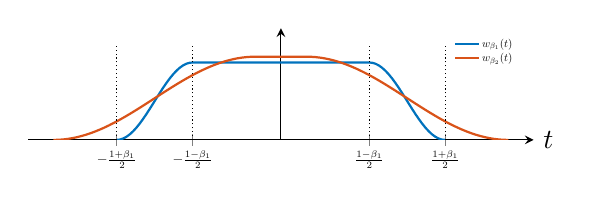
\begin{tikzpicture}[
declare function={
	func(\x,\b)= and(\x >= -(1-\b)/2, \x<= (1-\b)/2) * 2/sqrt(4-\b) + 
		       and(\x >= -(1+\b)/2, \x <= -(1-\b)/2) * 1/sqrt(4-\b)*(1+sin(deg(pi*(2*x+1)/(2*\b)))) +
		       and(\x >= (1-\b)/2, \x <= (1+\b)/2) * 1/sqrt(4-\b)*(1-sin(deg(pi*(2*x-1)/(2*\b)))) ;		       
},
]%
\begin{axis}[
  width = 8cm,
  height = 3cm,
  xlabel={$t$},
  axis x line=middle,  % Show only the x-axis
  axis y line=middle,    % Hide the y-axis
  xmin=-1, xmax=1,
  ymin=0, ymax=1.5,  % Set ymax to 2
  xtick={-0.65,-0.35,0.35,0.65},
  ytick=\empty,
  xticklabels={$-\frac{1+\beta_1}{2}$,$-\frac{1-\beta_1}{2}$,$\frac{1-\beta_1}{2}$,$\frac{1+\beta_1}{2}$},
  every tick label/.append style={scale=0.5},
  xlabel style={
    right,
  },
  legend style={draw=none,nodes={scale=0.4, transform shape}}
]%
\Tukeywindow{0.3}{0}{blue}
\addlegendentry{$w_{\beta_1}(t)$}
\Tukeywindow{0.8}{0}{red}
\addlegendentry{$w_{\beta_2}(t)$}
\addplot [black, densely dotted] coordinates {(-0.65,0)(-0.65,1.3)};
\addplot [black,  densely dotted] coordinates {(0.65,0)(0.65,1.3)};
\addplot [black,  densely dotted] coordinates {(0.35,0)(0.35,1.3)};
\addplot [black,  densely dotted] coordinates {(-0.35,0)(-0.35,1.3)};
\end{axis}%
\end{tikzpicture}%
\end{document}
























